\section*{Trees}

\label{sec:trees}

\vspace{5mm}

\textit{Intro} \\

We want to approximate $f: \mathcal{X} \to \mathcal{Y}$ where $\mathcal{Y}$ are the labels and $\mathcal{X}$ is the training set.

The objective is to partitionate $\mathcal{X}$ the best. At the start, $\mathcal{X}$ is the first node (root). \\

Training step: we build a tree that best classifies the training samples.

Predict step: we perform the tests of the tree that was built during the training step. \\

\textit{Impurity measure: Gini index} \\

To determine a good split element, we measure the impurity. One way to measure impurity is the Gini index. \\

\textbf{The Gini index is the probability of incorrectly classifying a random point}. Thus, a good separator has a \textbf{low} Gini index. \\

Mathematically, the Gini index $H$ (hyperplan) represents the disparity in a set $S$:

$$H(S)=\Sigma_{\ell=1}^C p_{\ell}(S)(1-p_{\ell}(S))$$

Or (easier to code): 
$$H(S)=\Sigma_{\ell=1}^C p_{\ell}(S)-\Sigma_{\ell=1}^C p_{\ell}(S)*p_{\ell}(S)=1-\Sigma_{\ell=1}^C p_{\ell}(S)^2$$

Where $p_{c}(S)=\frac{1}{n}\Sigma_{i=1}^n 1\{y_i=c\}$ is the frequency of label $c$ in a set $S$. $C$ is the set of labels. \\

\textit{Note}: if all elements belong to the same class, then it is called pure. Intuitively, to have more purity, we will favor a high count of elements in a small number of classes versus a low count of elements in a large number of classes. This is because $p_{\ell}(S)$ is at power $2$. E.g. $3^2 + 4^2 < 7^2 =>$ we prefer to have the 7 elements in the same class (more pure).\\

\begin{center}
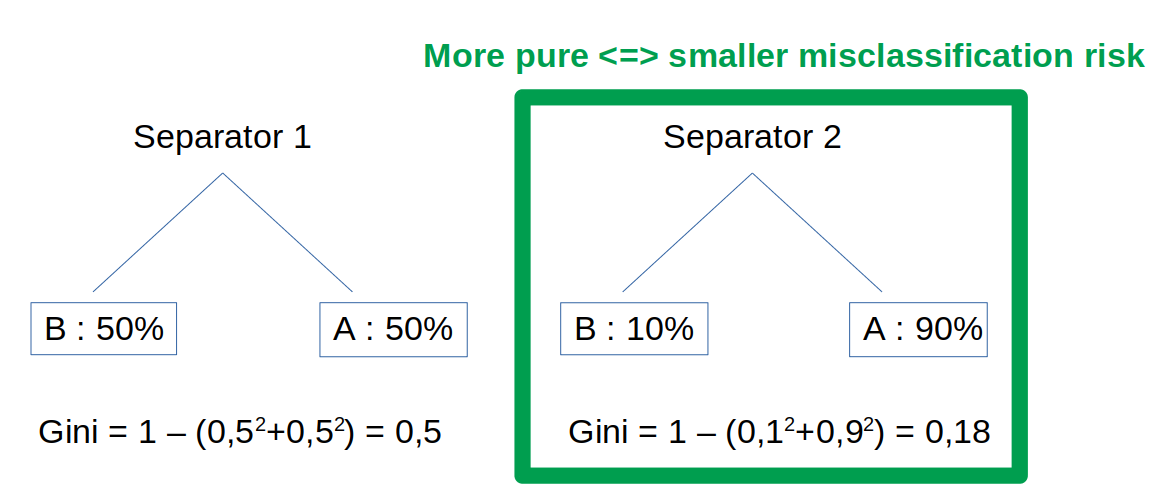
\includegraphics[scale=0.2]{tree_gini.png}
\end{center}

\textit{Loss function} \\

To assess the split quality, we use \textit{information gain} (= loss function) that compares the impurity (Gini index) between two trees. We compare the current tree with the one where we applied the split. The trees are weighted by the child importance.

$$\underset{j \in \{1,...,p\}, \\
\tau \in \mathbb{R}}{\operatorname{argmin}} \frac{n_r}{n}H(R(S,j,\tau))+\frac{n_l}{n}H(L(S,j,\tau))$$

$(j, \tau)$ are the possible feature values. $H()$ is the Gini index function as seen previously.

$R$ and $L$ are the Right and Left branches. We want a \textbf{low} disparity inside each of them. \\

\textit{Why linearity?} \\

$R(S,j,\tau)=\{(x,y), t_{j,\tau} \ge 0\}$ is the set of elements at the right of the node. The inequality $t_{j,\tau} \ge 0$ represents the split element which is a \textbf{linear separator}. Trees thus use several linear separators to build non linear decision functions. \\

\textit{Example} \\

In our example, we want to build a tree to classify client mandates the best as possible.

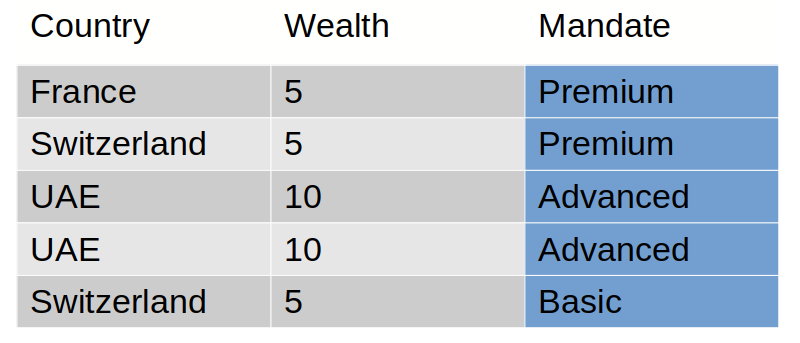
\includegraphics[scale=0.2]{trees_data.png}

The expected tree for this training set is:

\begin{center}
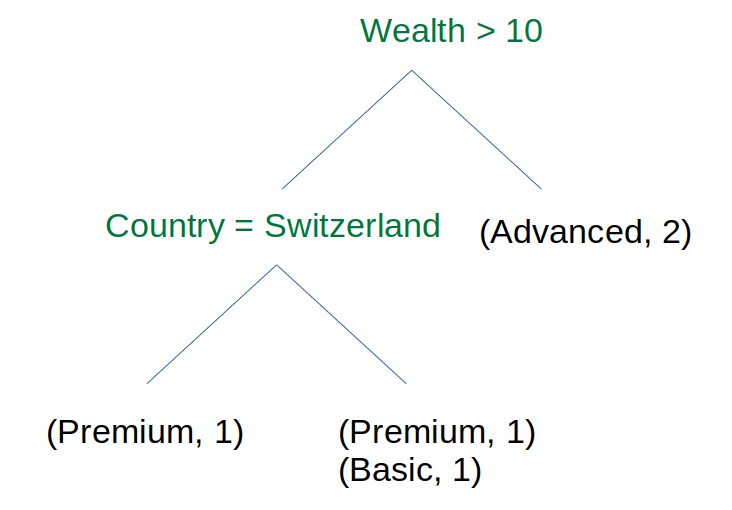
\includegraphics[scale=0.2]{trees_example.png}
\end{center}

The leafs are dictionaries of occurences. Those dictionaries can be used as a reliability measure for a prediction. E.g. if the client has a wealth < 10 and is located in Switzerland, there are 50-50\% chance that the client is Premium or Basic. \\

\textit{Algorithm} \\

The main steps of the algorithm are:

1. Loop on all features and values to find the element that best splits the data.\\
2. Create a partition thanks to this element. \\

3. Perform the same two first steps for the left and the right of the element. \\
4. Stop when you arrive to a Leaf. \\

The main function \textit{build\_tree()} is called recursively. 

\pagebreak

\begin{algorithm}
\caption{Trees}
\begin{algorithmic}
\Procedure{BUILD\_TREE(rows)}{}
\State gain, split\_element = FIND\_BEST\_SPLIT(rows)
\If{gain==0}
\State return Leaf(rows)
\EndIf
\State right\_rows, left\_rows = PARTITION(rows, split\_element)
\State right\_branch = BUILD\_TREE(right\_rows)
\State left\_branch = BUILD\_TREE(left\_rows)
\State return Decision\_Node(split\_element, right\_branch, left\_branch)
\EndProcedure
\end{algorithmic}
\end{algorithm}

A full implementation (largely inspired by \href{https://github.com/random-forests/tutorials/blob/master/decision_tree.ipynb}{Google tutorial}) can be found on my \href{https://github.com/savoga/various_projects/blob/master/trees_from_scratch.py}{github account}. \\

\textit{Important notes} \\

The final tree is a \textit{node}. Browsing the tree can be done as such: 

\textit{my\_tree.right\_branch.right\_branch.leaf}. 

This gives a dictionary of occurences for a branch with depth 3 (number of nodes). \\

The function FIND\_BEST\_SPLIT() loops on all features and all values to find the best split element. A split element is thus a couple (value, feature):

\begin{center}
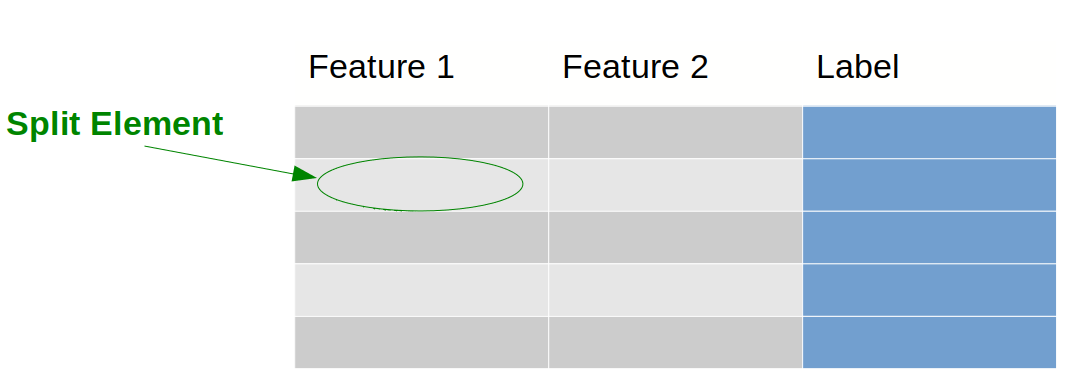
\includegraphics[scale=0.2]{trees_split_element.png}
\end{center}

The following tree illustrates the recursivity. In green are the \textit{split element}.

\begin{center}
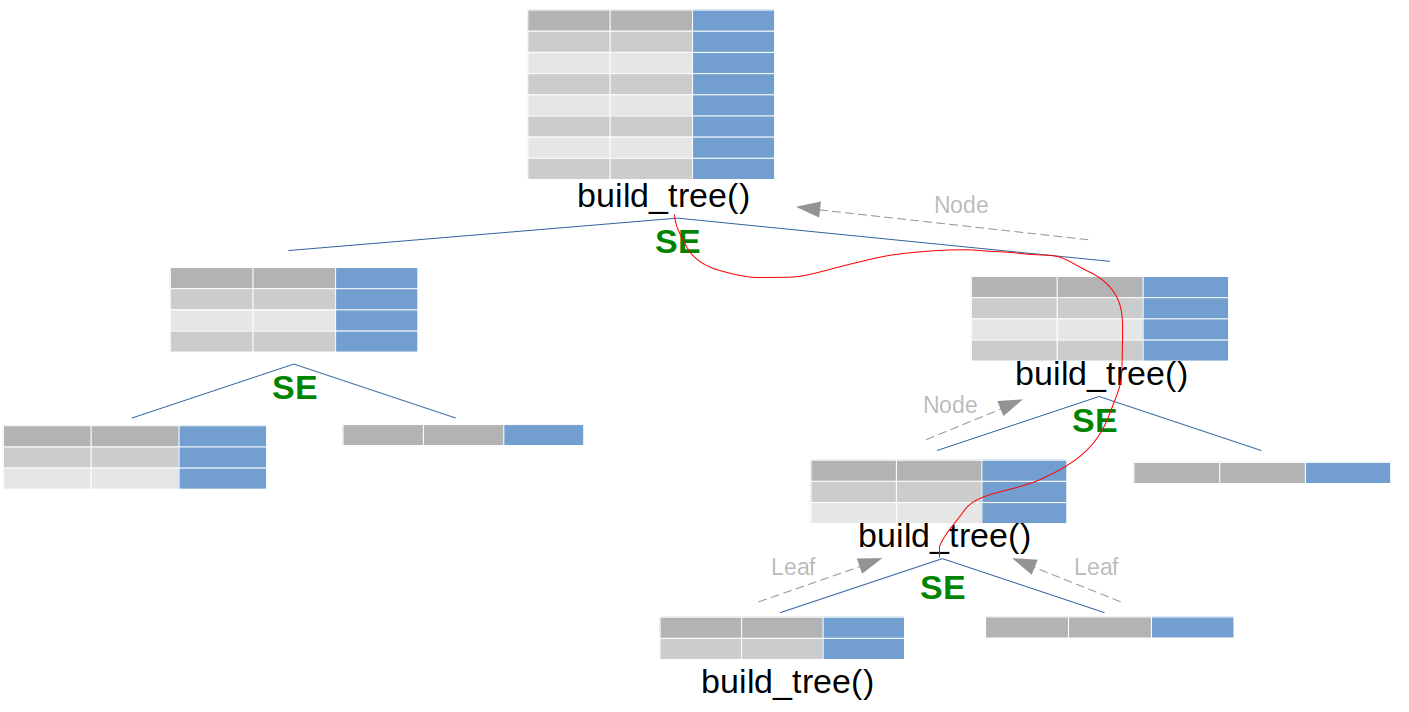
\includegraphics[scale=0.3]{trees_recursivity.png}
\end{center}

\textit{Variance} \\

Decision trees have a high variance meaning that the classification results can highly vary for different datasets. In other words, there is a high sensitivity to training data. If we draw Decision Trees for slightly different datasets (that we would however consider the same), we will have a large dispersion of the labels:

$$Var_m(y) = \frac{1}{M}\Sigma_{i=1}^M(y_i - \overline{y})^2$$

Where M are the considered datasets (almost similar) and $y_i$ are all the labels of one tree.

Intuitively, this problem lies in the hierarchy process of a tree: a small change in a node is echoed in every child nodes. \\

\textit{Feature importance} \\

\textit{scikit-learn} provides a \textit{feature\_importance\_} method associated with the Tree classifier. Feature importance is computed as such:

$$Node~Importance~(node) = NI(node) = \frac{N_t}{N}(Gini_t - \frac{N_{t,right}}{N_t}Gini_{right} - \frac{N_{t,left}}{N_t}Gini_{left})$$

The terms $\frac{N_t}{N}$,  $\frac{N_{t,right}}{N_t}$, $\frac{N_{t,left}}{N_t}$ are the probabilities to reach, respectively, the node we are interested in, its right child and left child.

$$Feature~Importance~(feat) = FI(node) = \frac{\Sigma_{k \in \text{ nodes with } \textit{feat } \text{as separator}}NI(node~k)}{\Sigma_{k \in \text{ all nodes}}NI(node~k)}$$

Example:

\begin{center}
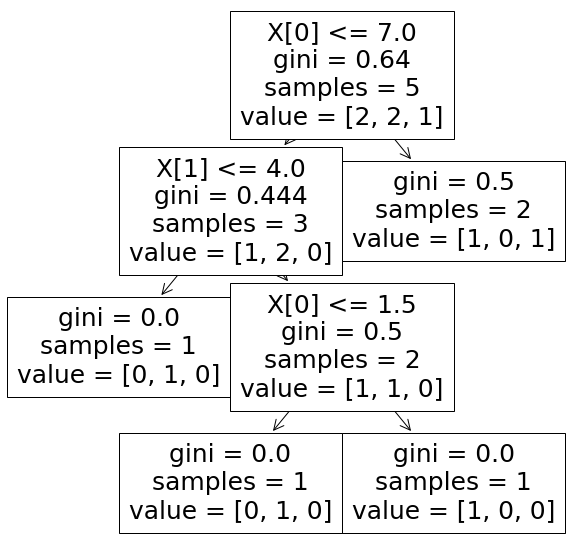
\includegraphics[scale=0.4]{tree_feat_importance.png}
\end{center}

$NI_0^{(1)} = \frac{5}{5}(0.64-\frac{2}{5}0.5-\frac{3}{5}*0.444) \approx 0.174$

$NI_0^{(2)} = \frac{3}{5}*(0.444-\frac{2}{3}*0.5-\frac{1}{3}*0) \approx 0.066$

$NI_1 = \frac{2}{5}*(0.5- \frac{1}{2}*0- \frac{1}{2}*0) \approx 0.2$ \\

$FI_0 = \frac{NI_0^{(1)} + NI_0^{(2)}}{NI_0^{(1)} + NI_0^{(2)} + NI_1} \approx 0.545$

$FI_1 = \frac{NI_1}{NI_0^{(1)} + NI_0^{(2)} + NI_1} \approx 0.454$ \\

The full code for this example can be found on my \href{https://github.com/savoga/various_projects/blob/master/trees_feature_importance.py}{Github account}.

\vspace{5mm}